% указываем класс документа
\documentclass[12pt,a4paper,openany]{extarticle}

% подключаем собственный стилевой файл 
\usepackage{mystyle}

% указываем язык (для автоматической вставки слов, типа "Глава", "Содержание", "Литература", "рис." и пр.
\selectlanguage{russian}

\begin{document}
\part*{Лабораторная работа №5\\
 Расчет коэффициентов регулятора на примере робота Segway}
\section{Методические рекомендации}
До начала работы студент должен выполнить предыдущие работы этого цикла. Необходимо знание методов модального управления.
\section{Теоретические сведения}
После того как мы получили матрицы состояния и управления для нашего робототехнического механизма, мы можем переходить к расчету регулятора. Для этого я приведу пример построения модального управления. Но это всего лишь один из немногих способов расчета регулятора, вы можете воспользоваться другими. Например, ПИ, ПИД или LQR регуляторами.\\ 
Во первых, нам нужно убедиться что наша система полностью управляема. Управляемость системы -- это свойство сисемы, описывающее возможность перевести ее из одного состояния в другое. Матрица управляемости $U=\begin{bmatrix} B & AB & A^2B & \dots & A^{n-1}B \end{bmatrix}$.\\
Теперь выберем эталонную матрицу. Эта матрица будет описывать нашу систему с регулятором, соответственно она должна быть устойчивой.

\begin{figure}[H]
	\noindent\centering{
		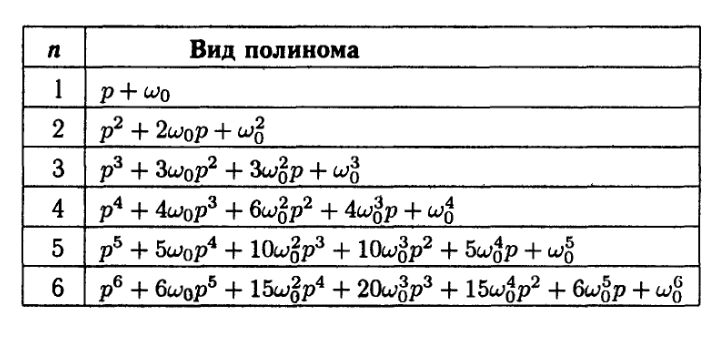
\includegraphics[scale=0.6]{Table1.png}
	}
	\caption{Биномиальное разложение.}
	\label{fig1}
\end{figure}
 Для выбора этой матрицы нам предлагается воспользоваться полиномами Ньютона или Баттерворта. Для нашей ситуации подойдет полином Ньютона, лишнее перерегулирование нам незачем. Так как у нас модель третьего порядка, а выбор полинома зависит от порядка системы, остановимся на этом $(p^3+3\omega_0p^2+3\omega_0^2p+\omega_0^3)y=u$.\\
Теперь нужно ответить на вопрос, что такое $\omega_0$. Значение этого параметра зависит от времени переходного процесса $t_\textit{п}^1$ при $\omega_0=1$, которое можно посмотреть в следующей таблице.

\begin{figure}[H]
	\noindent\centering{
		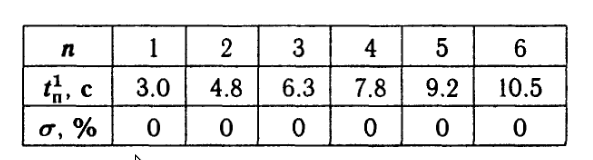
\includegraphics[scale=0.6]{Table2.png}
	}
	\caption{Качественные показатели.}
	\label{fig1}
\end{figure}

Для получения необходимого полинома нужно воспользоваться формулой $\omega_0=\cfrac{t_\textit{п}^1}{t_\textit{п}}$, а $t_\textit{п}$ следует выбирать в зависимости от интервала квантования вашей системы. В общем случае нужно выбрать значение равное 20 тактам. В зависимости от совершенства математической модели, это значение может изменяться.

\begin{figure}[H]
	\noindent\centering{
		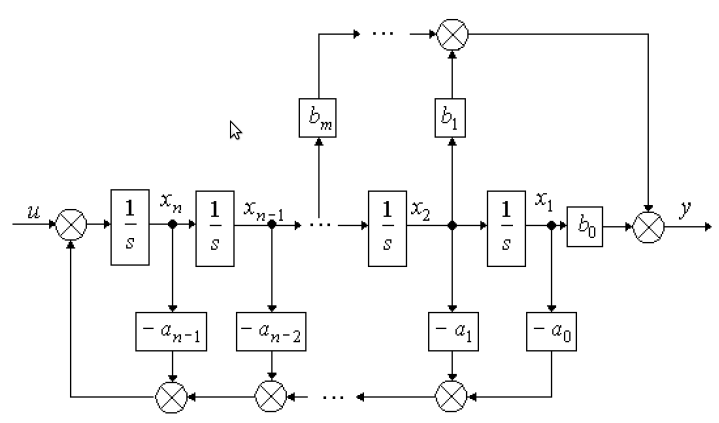
\includegraphics[scale=0.6]{Sheme1.png}
	}
	\caption{Представление полинома в канонической управляемой форме.}
	\label{fig1}
\end{figure}

Далее нужно воспользоваться представлением полученного эталонного полинома $(p^n+a_1p^{n-1}+\dots+a_{n-1}p+a_n)y=u$ в канонической управляемой форме.
\begin{equation}
\Gamma =
	\begin{bmatrix} 
		0 & 1 & 0 & \dots & 0\\
		0 & 0 & 1 & \dots & 0\\
		\hdotsfor{5}\\
		-a_n & -a_{n-1} & -a_{n-2} & \dots & -a_1 \\
	\end{bmatrix}
\end{equation}

Мы получили эталонную модель системы.

\begin{equation}
\left\{  
	\begin{array}{rcl}  
	\dot\xi & = & \xi\Gamma\\
	\nu & = & H\xi
	\end{array}   
	\right.,
\end{equation}

где $H$, матрица выхода эталонной модели. Выберем закон управления в виде $u=Kx$. После того как мы получили эталонную модель, мы можем составить уравнение, решением которого будет матрица коэффициентов обратной связи. 

\begin{equation}
A + BK = M\Gamma M^{-1}
\end{equation}

Домножим обе части на $M$, и получим следующее выражение:

\begin{equation}
-AM + M\Gamma = BKM,
\end{equation}

уравнение Сильвестра. Нам нужно замкнуть его, однозначно определив произведение матриц K*M. Для

\section{Цель работы}
Провести расчет регулятора и получить соответствующие коэффициенты. Практически реализовать систему и продемонстрировать ее работу.

\section{Порядок выполнения работы}
\begin{enumerate}
	\item Построение регулятора.
	\begin{enumerate}
		\item Из полученных матриц состояния и управления расчитайте регулятор.
		\item Занесите полученные данные в рограмму и проверьте их работоспособность.
	\end{enumerate}
	\item Обработка данных.
	\begin{enumerate}
		\item Выведите графики управляющего воздействия и состояния объекта.
	\end{enumerate}
\end{enumerate}
\section{Содержание отчета}
\begin{enumerate}
	\item Вывод математической модели объкта.
	\item Описание объекта в~пространстве состояния.
	\item Схема моделирования и график, полученные при~математическом моделировании.
\end{enumerate}
\end{document}

\end{document}